% Please do not change the document class
\documentclass{scrartcl}

% Please do not change these packages
\usepackage[hidelinks]{hyperref}
\usepackage[none]{hyphenat}
\usepackage{setspace}
\usepackage{graphicx}
\graphicspath{ {C:/Users/james/Documents/GitHub/comp150-desktop-game-Eval/Figures/} }
\doublespace

% You may add additional packages here
\usepackage{amsmath}

% Please include a clear, concise, and descriptive title
\title{Evaluation}

% Please do not change the subtitle
\subtitle{COMP150 - Evaluation}

% Please put your student number in the author field
\author{1506530}

\begin{document}

\maketitle

\section{Group Overview}
\begin{figure}[h]
	\centering
	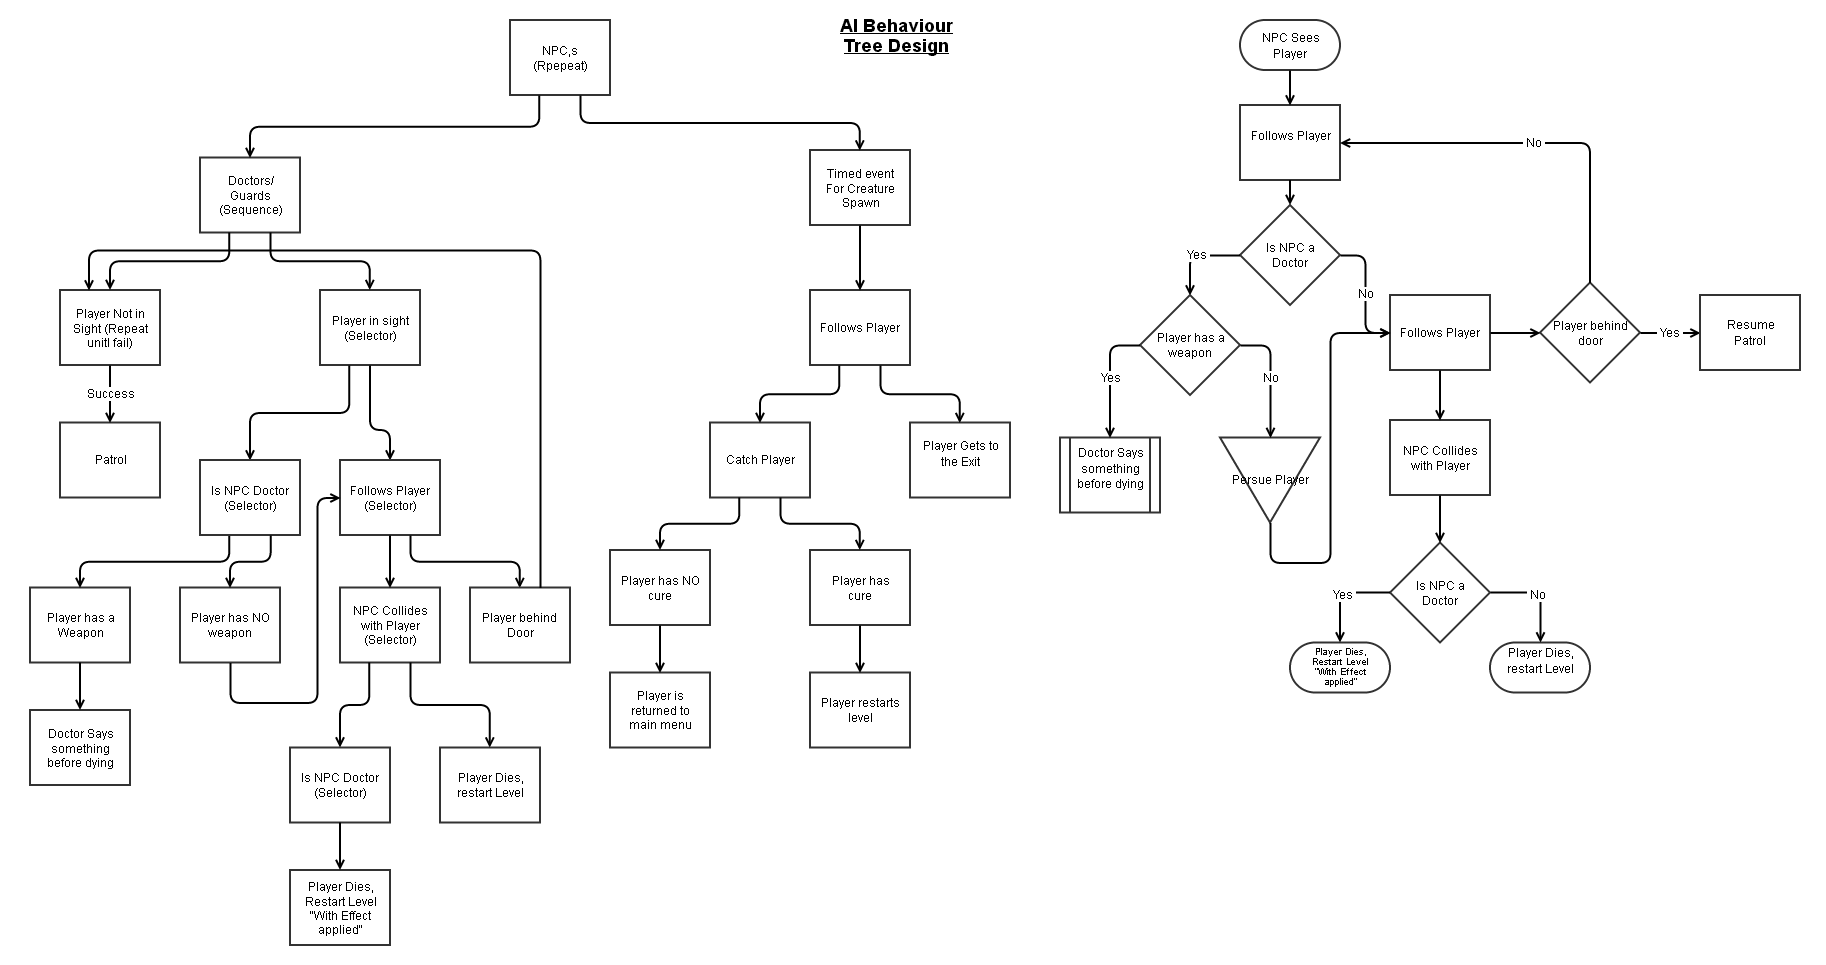
\includegraphics[width=0.7\linewidth]{ai_behaviour_tree}
	\caption{ - Original Design For The AI }.
	\label{ai_behaviour_tree}
\end{figure}

During the weeks of creating this game I have learned a substantial amount on not only teamwork but the use of different software's. As a group we faced challenges that impeded our work flow considerably, among these were for me self-motivation, asking for help and lack of understanding of the code presented. Our game is a simple 2D topdown style maze game, as can be seen by figure one it consisted of a maze some NPC's and the player. The goal is to make it to the end without being caught by an NPC. Originally as can be seen by figure two the AI for the game was intended to be far more complex, although time constraints required us to remove aspects of the AI. This along with many other user stories for the game were not implemented sue to the time constraints.

\section{Working Collaboratively In Person and Self Motivation}
When the project started I felt confident in our ability to for fill all of the user stories, but as time went on that confidence waned. In the first few weeks the game architecture was set-up, I then moved in to add the sprites and begin my work on the NPC's, this was done through pair programming. I believe that pair programming is essential to the success of any project as this allows two programmers to work co As a group we tried several different ways to communicate and work together on the same screen at the same time\cite{Radermacher:2011:IEI:1953163.1953346}. Unfortunately this did not last, it seems that with the current set-up for studio the group was not as motivated to come in to work together as was needed. This cost the game valuable collaborative time, issues like this are bound to rise when working with a variety of people with limited equipment. 
\newline
As the project went on I found that I was struggling to keep my motivation at its peak, there are several reasons for this. One reason was every time I attempted to solve an issue in the game I felt as though I was clashing with a brick wall. Relating to the first point, I work better with a group in person rather than on my own as the physical presence of others helps to keep me focused. Also my lack of communication with the others for example ``not asking question when questions are needed'', hindered my productivity. Being separated from my group gave the feeling as though I was a one man group, trying to work on the project without assistance. This being a personal issue, as I was well aware that I was not the only one working on the game, still caused me to struggle with productivity. A viable solution to this would be having predefined working days and setting up screen sharing and online calls. Doing this will allow everyone to stay at home while having the ability to communicate instantaneously with one another. 

\section{Scope}
The game was over scoped. We initially thought we could achieve far more for the game than was possible for the skills and time we had. This caused a higher level of stress and feeling of being a bit lost in the group. As we went on and the backlog seemed to never end, the groups moral suffered, and we began to fall behind on our work. In turn this caused the scope of the game to be even further out of reach. Towards the end of our sprints we decided to be as optimistic as possible about the situation and cut several features from the game. This brought the game back into scope and we are nearing completion. The issue here was that we did not take into account possible absences, personal struggles and/or preferred place of work. If we had taken these possible issues into account we could have solved them by organising our group better and being honest about what workload people could handle, this would have helped to keep the game within scope. Also a slight under scoping would have proved beneficial, as, is someone was unexpectedly absent we could have still achieved our final goal.

\section{Final Remarks}
I have learnt a lot about working in a group of equals during my time one this project, as I am traditionally used to having a single authoritative figure in charge of everything. I believe these lessons will help me to organise myself better for future projects and prevent any of these issues arising again. 


\bibliographystyle{ieeetran}
\bibliography{COMP150-Group_Eval}

\end{document}